\documentclass{beamer}

\usepackage[utf8]{inputenc}
\usepackage[russian]{babel}

\usepackage{listings}
\usepackage{hyperref}

\lstdefinelanguage{scala}{
  morekeywords={abstract,case,catch,class,def,%
    do,else,extends,false,final,finally,%
    for,if,implicit,import,match,mixin,%
    new,null,object,override,package,%
    private,protected,requires,return,sealed,%
    super,this,throw,trait,true,try,%
    type,val,var,while,with,yield},
  otherkeywords={=>,<-,<\%,<:,>:,\#,@},
  sensitive=true,
  morecomment=[l]{//},
  morecomment=[n]{/*}{*/},
  morestring=[b]",
  morestring=[b]',
  morestring=[b]"""
}

\mode<presentation> {

% The Beamer class comes with a number of default slide themes
% which change the colors and layouts of slides. Below this is a list
% of all the themes, uncomment each in turn to see what they look like.

%\usetheme{default}
%\usetheme{AnnArbor}
%\usetheme{Antibes}
%\usetheme{Bergen}
%\usetheme{Berkeley}
%\usetheme{Berlin}
%\usetheme{Boadilla}
%\usetheme{CambridgeUS}
%\usetheme{Copenhagen}
%\usetheme{Darmstadt}
%\usetheme{Dresden}
%\usetheme{Frankfurt}
%\usetheme{Goettingen}
%\usetheme{Hannover}
%\usetheme{Ilmenau}
%\usetheme{JuanLesPins}
%\usetheme{Luebeck}
\usetheme{Madrid}
%\usetheme{Malmoe}
%\usetheme{Marburg}
%\usetheme{Montpellier}
%\usetheme{PaloAlto}
%\usetheme{Pittsburgh}
%\usetheme{Rochester}
%\usetheme{Singapore}
%\usetheme{Szeged}
%\usetheme{Warsaw}

% As well as themes, the Beamer class has a number of color themes
% for any slide theme. Uncomment each of these in turn to see how it
% changes the colors of your current slide theme.

%\usecolortheme{albatross}
%\usecolortheme{beaver}
%\usecolortheme{beetle}
%\usecolortheme{crane}
%\usecolortheme{dolphin}
%\usecolortheme{dove}
%\usecolortheme{fly}
%\usecolortheme{lily}
%\usecolortheme{orchid}
%\usecolortheme{rose}
%\usecolortheme{seagull}
%\usecolortheme{seahorse}
%\usecolortheme{whale}
%\usecolortheme{wolverine}

%\setbeamertemplate{footline}
%\setbeamertemplate{footline}[page number]

%\setbeamertemplate{navigation symbols}{}
}

\usepackage{graphicx} % Allows including images
\usepackage{booktabs} % Allows the use of \toprule, \midrule and \bottomrule in tables

\title[отладчик типов scala]{Отладчик вывода типов языка программирования Scala в intellij idea}

\author[Роман Васильев]{
Роман Васильев \\ руководитель: Александр Подхалюзин
}
\institute[АУ]
{
Академический университет
% \medskip
% \textit{john@smith.com} % Your email address
}
\date{\today}

\begin{document}

\begin{frame}
\titlepage
\end{frame}

% \begin{frame}
% \frametitle{Overview}
% \tableofcontents
% \end{frame}

% \section{First Section}
%
% \subsection{Subsection Example}

\begin{frame}
\frametitle{Введение}
\begin{block}{Система типов}
«Система типов - это гибко управляемый синтаксический метод
доказательства отсутствия в программе определенных видов по-
ведения при помощи классификации выражений языка по разно-
видностям вычисляемых ими значений».
\end{block}

Система типов в языке программирования Scala
\begin{itemize}
  \item Статическая
  \item Строгая
  \item С выводом типов
\end{itemize}
\end{frame}

\begin{frame}
\frametitle{Рассматриваемые процессы}
\begin{itemize}
  \item Проверка сводимости типов.
  % Есть ожидаемый тип, есть выражение, нужно проверить что тип выражаение удовлетворяет ожидаемому типу.
  \item Вывод типов.
  % Следует из сводиомсти типов. Осмысленно в рамках полиморфных функций.
  \item Выбор перегрузки.
  %  Несколько функций с одинаковыми названиями.
\end{itemize}
\end{frame}

\begin{frame}
\frametitle{Спецификация Scala}
\begin{itemize}
  \item Сводимость вводиться как отношение соответствующее транзитивному замыканию над набором правил вывода.
  \item Локальный вывод типов:
  \begin{itemize}
    \item $expr.x$
    \item $expr$
    \item $expr(d_1,..., d_m)$
  \end{itemize}
  \item Разрешение перегрузки сначала пытается отсеить кандидатов не обращаясь к конкретным переданным аргументам.
  После этого идет выбор наиболее специфичного представителя.
  % рассказать про shape
\end{itemize}
\end{frame}

\begin{frame}
\frametitle{Существующее решение}
Scala type debugger
\footnote{\scriptsize{\url{https://github.com/hubertp/prefuse-type-debugger}}}
\footnote{\scriptsize{\url{https://infoscience.epfl.ch/record/179877/files/typedebugger-applc2012.pdf}}}
использует инфраструктуру логгирования компилятора scala для сбора информации
и библиотекой prefuse для пользовательского интерфейса.

\vfill

Проблемы:
\begin{itemize}
  \item Используется специальная, инструментированная версия компилятора.
  \item Последний коммит в 2012.
\end{itemize}
\end{frame}

% необходимость какой-то реализации как основы

\begin{frame}
\frametitle{Цель и задачи}
Сделать отладчик механизмов связанных с типами в Scala Plugin
\begin{itemize}
  \item Инструментировать Scala Plugin для сбора промежуточной информации
  \item Дать интерпретацию с точки зрения спецификации scala
  \item Уменьшить влияние инструментации во время выполнения
\end{itemize}
\end{frame}

\begin{frame}
\frametitle{Архитектура}
\begin{center}
  \makebox[\textwidth]{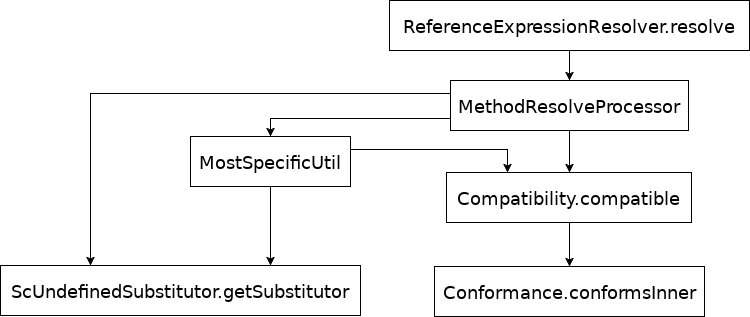
\includegraphics[width=0.9\paperwidth]{call-graph}}
\end{center}
\end{frame}


\defverbatim[colored]\realExample{
\begin{lstlisting}[language=scala,basicstyle=\ttfamily,keywordstyle=\color{red}]
@uninstrumental("handler")
case class MostSpecificUtil(
  elem: PsiElement,
  length: Int,
  handler: Option[DCHandler.Resolver] = None
)(implicit typeSystem: TypeSystem)
\end{lstlisting}
}

\defverbatim[colored]\originFunction{
\begin{lstlisting}[language=scala,basicstyle=\ttfamily,keywordstyle=\color{red},frame=single]
def f(..., h: Option[H])
\end{lstlisting}
}

% про то что одновременно хочется сохранять структуры используемые программой
% и при этом чтобы во время выполнения этих структур не было
\begin{frame}
\frametitle{Инструментирование и макросы}
\begin{itemize}
  \item def f(..., h: Option[H]) $\to$ def f(...); def f\$I(..., h: Option[H])
  \item class F(..., h: Option[H]) $\to$ class F(...); object F.\$I(..., h: Option[H])
\end{itemize}
\realExample
\end{frame}


\begin{frame}
\frametitle{Сложности}
\begin{itemize}
  \item Scala
  \item Несоответствие сущностей используемых в плагине и в документации скалы.
  Частая необходимость в обратном анализе.
  \item Наглядный пользовательский интерфейс.
  \item Работа с макросами. Трудность отладки. % про классы.
\end{itemize}
\end{frame}

\begin{frame}
\frametitle{Пример}
\makebox[\textwidth]{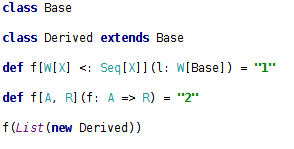
\includegraphics[width=0.9\paperwidth]{example}}
\end{frame}

\begin{frame}
\frametitle{Результат 1}
\makebox[\textwidth]{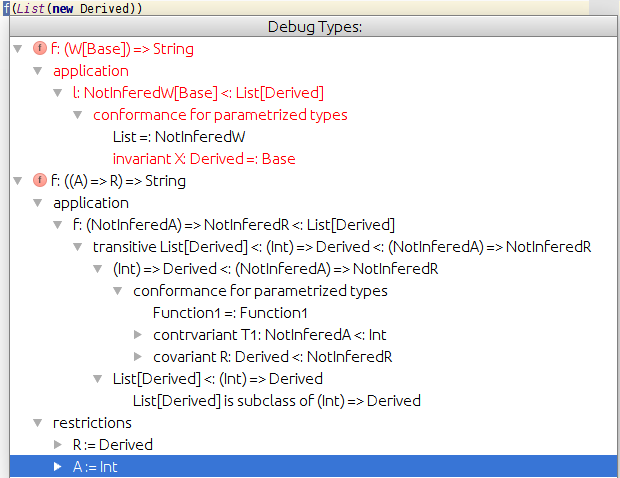
\includegraphics[width=0.9\paperwidth]{result1}}
\end{frame}

\begin{frame}
\frametitle{Результат 2}
\makebox[\textwidth]{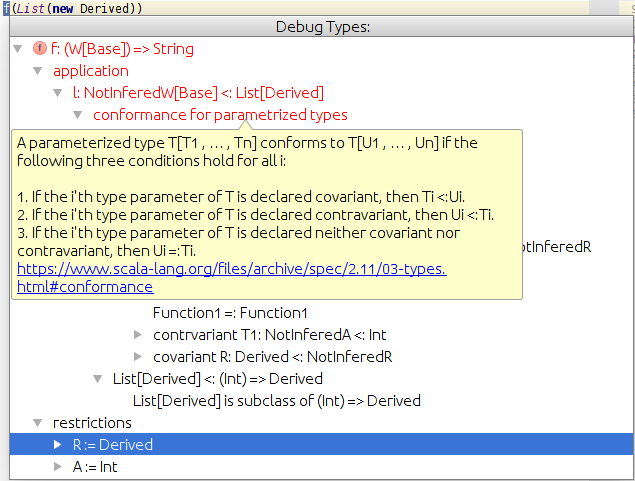
\includegraphics[width=0.9\paperwidth]{result2}}
\end{frame}

\begin{frame}
\frametitle{Результат 3}
\makebox[\textwidth]{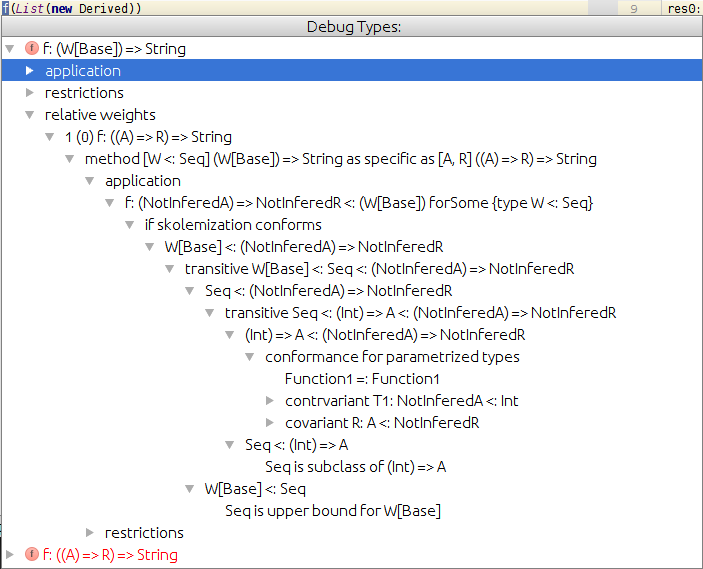
\includegraphics[width=0.9\paperwidth]{result3}}
\end{frame}

\begin{frame}
\frametitle{Репозиторий}
Код можно посмотреть здесь
\url{https://github.com/nizshee/intellij-scala}
\end{frame}

\begin{frame}
\Huge{\centerline{Конец}}
\end{frame}


%------------------------------------------------
%
% \begin{frame}
% \frametitle{Blocks of Highlighted Text}
% \begin{block}{Block 1}
% Lorem ipsum dolor sit amet, consectetur adipiscing elit.
% \end{block}
%
% \begin{block}{Block 2}
% Pellentesque sed tellus purus.
% \end{block}
%
% \begin{block}{Block 3}
% Suspendisse tincidunt sagittis gravida.
% \end{block}
% \end{frame}
%
% %------------------------------------------------
%
% \begin{frame}
% \frametitle{Multiple Columns}
% \begin{columns}[c]
%
% \column{.45\textwidth} % Left column and width
% \textbf{Heading}
% \begin{enumerate}
% \item Statement
% \item Explanation
% \item Example
% \end{enumerate}
%
% \column{.5\textwidth}
% Lorem ipsum dolor sit amet, consectetur adipiscing elit.
%
% \end{columns}
% \end{frame}
%
% %------------------------------------------------
% \section{Second Section}
% %------------------------------------------------
%
% \begin{frame}
% \frametitle{Table}
% \begin{table}
% \begin{tabular}{l l l}
% \toprule
% \textbf{Treatments} & \textbf{Response 1} & \textbf{Response 2}\\
% \midrule
% Treatment 1 & 0.0003262 & 0.562 \\
% Treatment 2 & 0.0015681 & 0.910 \\
% Treatment 3 & 0.0009271 & 0.296 \\
% \bottomrule
% \end{tabular}
% \caption{Table caption}
% \end{table}
% \end{frame}
%
% \begin{frame}
% \frametitle{Theorem}
% \begin{theorem}[Mass--energy equivalence]
% $E = mc^2$
% \end{theorem}
% \end{frame}
%
% \begin{frame}[fragile] % Need to use the fragile option when verbatim
% \frametitle{Verbatim}
% \begin{example}[Theorem Slide Code]
% \begin{verbatim}
% \begin{frame}
% \frametitle{Theorem}
% \begin{theorem}[Mass--energy equivalence]
% $E = mc^2$
% \end{theorem}
% \end{frame}\end{verbatim}
% \end{example}
% \end{frame}
%
% \begin{frame}
% \frametitle{Figure}
% Uncomment the code on this slide to include your own image from the same
% %\begin{figure}
% %\includegraphics[width=0.8\linewidth]{test}
% %\end{figure}
% \end{frame}
%
% \begin{frame}[fragile] % Need to use the fragile option when verbatim
% \frametitle{Citation}
% An example of the \verb|\cite| command to cite within the presentation:\\~
%
% This statement requires citation \cite{p1}.
% \end{frame}
%
% \begin{frame}
% \frametitle{References}
% \footnotesize{
% \begin{thebibliography}{99} % Beamer does not support BibTeX so references
% \bibitem[Smith, 2012]{p1} John Smith (2012)
% \newblock Title of the publication
% \newblock \emph{Journal Name} 12(3), 45 -- 678.
% \end{thebibliography}
% }
% \end{frame}

\end{document}
